\documentclass[12pt]{article}
\usepackage{amsmath, amssymb}
\usepackage{graphicx}
\usepackage{enumitem}
\usepackage[margin=1in]{geometry}

\begin{document}

\begin{center}
    {\LARGE \textbf{GATE -2015 MT}}\\[1em]
    ai25btech11009 \qquad Dasu Harshith Kumar
\end{center}

\begin{enumerate}

\item Choose the appropriate word/phrase, out of the four options given below, to complete the following sentence:\\
Apparent lifelessness ---  dormant life. (GATE 2015 MT)

\vspace{0.5em}
\begin{enumerate}[label=(\alph*)]
    \item harbours
    \item leads to
    \item supports
    \item affects
\end{enumerate}
\vspace{0.5em}

\item Fill in the blank with the correct idiom/phrase. That boy from the town was a --- in the sleepy village. (GATE 2015 MT)

\vspace{0.5em}
\begin{enumerate}[label=(\alph*)]
    \item dog out of herd
    \item sheep from the heap
    \item fish out of water
    \item bird from the flock
\end{enumerate}
\vspace{0.5em}

\item Choose the statement where underlined word is used correctly. (GATE 2015 MT)

\vspace{0.5em}
\begin{enumerate}[label=(\alph*)]
    \item When the teacher eludes to different authors, he is being elusive.
    \item When the thief keeps eluding the police, he is being elusive.
    \item Matters that are difficult to understand, identify or remember are allusive.
    \item Mirages can be allusive, but a better way to express them is illusory.
\end{enumerate}
\vspace{0.5em}

\item Tanya is older than Eric. Cliff is older than Tanya. Eric is older than Cliff. If the first two statements are true, then the third statement is: (GATE 2015 MT)

\vspace{0.5em}
\begin{enumerate}[label=(\alph*)]
    \item True
    \item False
    \item Uncertain
    \item Data insufficient
\end{enumerate}
\vspace{0.5em}

\item Five teams have to compete in a league, with every team playing every other team exactly once, before going to the next round. How many matches will have to be held to complete the league round of matches? (GATE 2015 MT)

\vspace{0.5em}
\begin{enumerate}[label=(\alph*)]
    \item 20
    \item 10
    \item 8
    \item 5
\end{enumerate}
\vspace{0.5em}

\item Select the appropriate option in place of underlined part of the sentence. Increased productivity necessary reflects greater efforts made by the employees. (GATE 2015 MT)

\vspace{0.5em}
\begin{enumerate}[label=(\alph*)]
    \item Increase in productivity necessary
    \item Increase productivity is necessary
    \item Increase in productivity necessarily
    \item No improvement required
\end{enumerate}
\vspace{0.5em}

\item Given below are two statements followed by two conclusions. Assuming these statements to be true, decide which one logically follows.\\
Statements: I. No manager is a leader. II. All leaders are executives.\\
Conclusions: I. No manager is an executive. II. No executive is a manager. (GATE 2015 MT)

\vspace{0.5em}
\begin{enumerate}[label=(\alph*)]
    \item Only conclusion I follows.
    \item Only conclusion II follows.
    \item Neither conclusion I nor II follows.
    \item Both conclusions I and II follow.
\end{enumerate}
\vspace{0.5em}

\item In the given figure, angle Q is a right angle, PS:QS = 3:1, RT:QT = 5:2 and PU:UR = 1:1. If area of triangle QTS is 20 cm$^2$, then the area of triangle PQR in cm$^2$ is ----. (GATE 2015 MT)

\vspace{0.5em}
\begin{center}
    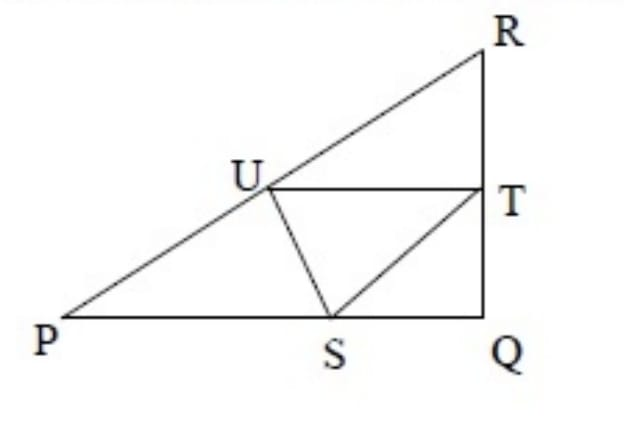
\includegraphics[width=0.5\textwidth]{images/q8i.jpg}
\end{center}
\vspace{0.5em}

\item Right triangle PQR is to be constructed in the $xy$-plane so that the right angle is at P and line PR is parallel to the $x$-axis. The $x$ and $y$ coordinates of P, Q, and R are to be integers that satisfy the inequalities: $-4\leq x \leq 5$ and $6 \leq y \leq 16$. How many different triangles could be constructed with these properties? (GATE 2015 MT)

\vspace{0.5em}
\begin{enumerate}[label=(\alph*)]
    \item 110
    \item 1,100
    \item 9,900
    \item 10,000
\end{enumerate}
\vspace{0.5em}

\item A coin is tossed thrice. Let X be the event that head occurs in each of the first two tosses. Let Y be the event that a tail occurs on the third toss. Let Z be the event that two tails occur in three tosses. Based on the above information, which one of the following statements is TRUE? (GATE 2015 MT)

\vspace{0.5em}
\begin{enumerate}[label=(\alph*)]
    \item X and Y are not independent
    \item Y and Z are dependent
    \item Y and Z are independent
    \item X and Z are independent
\end{enumerate}
\vspace{0.5em}

\item The standard deviation of the readings 19, 17, 15, 13, 11 is ----. (GATE 2015 MT)

\vspace{0.5em}

\item $\frac{y(x+h)-y(x)}{h}$ is a numerical approximation for (GATE 2015 MT)

\vspace{0.5em}
\begin{enumerate}[label=(\alph*)]
    \item $\frac{dy}{dx}$
    \item $\frac{dy}{dh}$
    \item $\int y dx$
    \item $\int x dy$
\end{enumerate}
\vspace{0.5em}

\item If A and B are matrices, $(AB)^T =$ (GATE 2015 MT)

\vspace{0.5em}
\begin{enumerate}[label=(\alph*)]
    \item $A^T B$
    \item $B^T A$
    \item $A^T B^T$
    \item $B^T A^T$
\end{enumerate}
\vspace{0.5em}

\item Which of the following properties is intensive? (GATE 2015 MT)

\vspace{0.5em}
\begin{enumerate}[label=(\alph*)]
    \item Volume
    \item Gibbs free energy
    \item Chemical potential
    \item Entropy
\end{enumerate}
\vspace{0.5em}

\item In an Ellingham diagram, the standard free energy change $\Delta G^\circ$ for the oxidation reaction of a metal M is plotted as a function of temperature. The slope of this line is positive because (GATE 2015 MT)

\vspace{0.5em}
\begin{enumerate}[label=(\alph*)]
    \item $\Delta S^\circ$ is positive
    \item $\Delta S^\circ$ is negative
    \item $\Delta H^\circ$ is positive
    \item $\Delta H^\circ$ is negative
\end{enumerate}
\vspace{0.5em}

\item In froth flotation, hydrophobic mineral particles ascend with air bubbles preferentially over hydrophilic mineral particles. The figure below shows a schematic of a water droplet placed on the surfaces of two mineral P and Q. (GATE 2015 MT)

\vspace{0.5em}
\begin{center}
    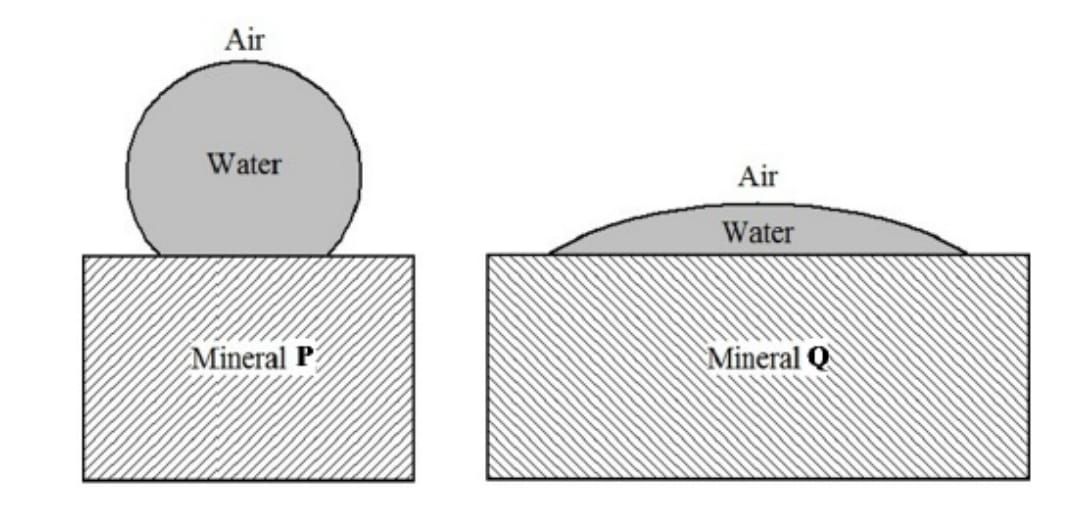
\includegraphics[width=0.55\textwidth]{images/q16i.jpg}
\end{center}
\begin{enumerate}[label=(\alph*)]
    \item Mineral P ascends with air bubbles preferentially over mineral Q.
    \item Mineral Q ascends with air bubbles preferentially over mineral P.
    \item Both minerals P and Q ascend with the air bubbles without preference.
    \item Both minerals P and Q sink to the bottom.
\end{enumerate}
\vspace{0.5em}

\item Which of the following oxide addition results in polymerization (i.e., network formation) in a silicate slag? (GATE 2015 MT)

\vspace{0.5em}
\begin{enumerate}[label=(\alph*)]
    \item CaO
    \item MgO
    \item P$_2$O$_5$
    \item Na$_2$O
\end{enumerate}
\vspace{0.5em}

\item Zn is commercially extracted from which of the following minerals? (GATE 2015 MT)

\vspace{0.5em}
\begin{enumerate}[label=(\alph*)]
    \item Sphalerite
    \item Magnetite
    \item Chalcopyrite
    \item Galena
\end{enumerate}
\vspace{0.5em}

\item Self supporting arches for furnace roofs can be fabricated using silica bricks but not using magnesia bricks. Why? (GATE 2015 MT)

\vspace{0.5em}
\begin{enumerate}[label=(\alph*)]
    \item Silica has a significantly lower thermal expansion coefficient than magnesia at high temperatures.
    \item Silica has a significantly higher thermal conductivity than magnesia at high temperatures.
    \item Silica has a significantly lower melting point than magnesia.
    \item Silica is significantly more acidic than magnesia.
\end{enumerate}
\vspace{0.5em}

\item A species can diffuse through the lattice (diffusion coefficient, $D_L$), along grain boundaries (diffusion coefficient, $D_{GB}$), and along free surfaces (diffusion coefficient, $D_S$). Which of the following relations is CORRECT? (GATE 2015 MT)

\vspace{0.5em}
\begin{enumerate}[label=(\alph*)]
    \item $D_L > D_{GB} > D_S$
    \item $D_S > D_L > D_{GB}$
    \item $D_{GB} > D_S > D_L$
    \item $D_S > D_{GB} > D_L$
\end{enumerate}
\vspace{0.5em}

\item Select the CORRECT plot of Gibbs free energy $(G)$ vs temperature $(T)$ for a single component system from the following: (GATE 2015 MT)

\vspace{0.5em}
\begin{center}
    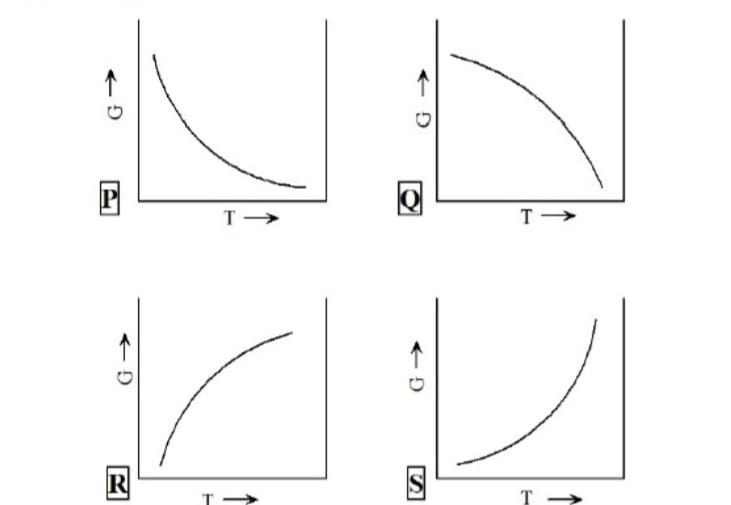
\includegraphics[width=0.45\textwidth]{images/q21i.jpg}
\end{center}
\begin{enumerate}[label=(\alph*)]
    \item P
    \item Q
    \item R
    \item S
\end{enumerate}
\vspace{0.5em}

\item If $A_x$ represents adherent oxide layer thickness and $t$ is time, which of the following curves represents diffusion-controlled oxidation kinetics? (GATE 2015 MT)

\vspace{0.5em}
\begin{center}
    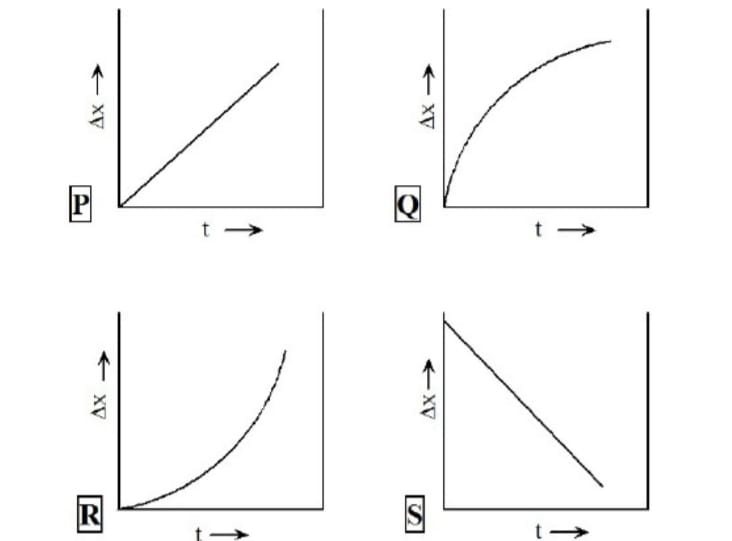
\includegraphics[width=0.45\textwidth]{images/q22i.jpg}
\end{center}
\begin{enumerate}[label=(\alph*)]
    \item P
    \item Q
    \item R
    \item S
\end{enumerate}
\vspace{0.5em}

\item Based on the standard galvanic series, select the CORRECT sequence of metals in the increasing order of anodic behaviour: (GATE 2015 MT)

\vspace{0.5em}
\begin{enumerate}[label=(\alph*)]
    \item Zn, Fe, Pt, Cu
    \item Pt, Zn, Cu, Fe
    \item Fe, Pt, Cu, Zn
    \item Pt, Cu, Fe, Zn
\end{enumerate}
\vspace{0.5em}

\item In a conventional unit cell of a crystal, $a = b = c$ and $\alpha = \beta = \gamma = 90^\circ$. This crystal belongs to which of the following systems? (GATE 2015 MT)

\vspace{0.5em}
\begin{enumerate}[label=(\alph*)]
    \item Cubic
    \item Tetragonal
    \item Orthorhombic
    \item Triclinic
\end{enumerate}
\vspace{0.5em}

\item In an X-ray powder pattern of a simple cubic crystal, the 2nd peak corresponds to (GATE 2015 MT)

\vspace{0.5em}
\begin{enumerate}[label=(\alph*)]
    \item (111)
    \item (100)
    \item (200)
    \item (110)
\end{enumerate}
\vspace{0.5em}

\item  When boron (trivalent) is doped into silicon, the resulting material is (GATE 2015 MT)
\begin{enumerate}[label=(\alph*)]
  \item a p-type semiconductor.
  \item an n-type semiconductor.
  \item a superconductor.
  \item an insulator.
\end{enumerate}

\item  Which of the following metal working operations is categorized as an indirect compression process? (GATE 2015 MT)
\begin{enumerate}[label=(\alph*)]
  \item Forging
  \item Wire drawing
  \item Extrusion
  \item Stretch forming
\end{enumerate}

\item  Which of the following is a typical rolling defect? (GATE 2015 MT)
\begin{enumerate}[label=(\alph*)]
  \item Buckling
  \item Edge cracking
  \item Cold shut
  \item Porosity
\end{enumerate}

\item Which manufacturing process is NOT used for producing fine-grained metals? (GATE 2015 MT)
\begin{enumerate}[label=(\alph*)]
  \item Electrodeposition
  \item Czochralski method
  \item Equi-Channel Angular Pressing (ECAP)
  \item Sintering of milled powders
\end{enumerate}

\item  Which metal forming technique is used for making soft drink cans from aluminum sheets? (GATE 2015 MT)
\begin{enumerate}[label=(\alph*)]
  \item Rolling
  \item Forging
  \item Deep drawing
  \item Extrusion
\end{enumerate}

\item  Which of the following is NOT a solid state metal joining technique? (GATE 2015 MT)
\begin{enumerate}[label=(\alph*)]
  \item Ultrasonic welding
  \item Friction welding
  \item Diffusion bonding
  \item Electroslag welding
\end{enumerate}

\item  The stress required for Orowan dislocation bypass is 200 MPa at a 500 nm inter-precipitate spacing. At 200 nm spacing, the required stress is approximately (GATE 2015 MT)


\item  Which Mohr's circle represents equi-biaxial tension? (GATE 2015 MT)
\begin{center}
  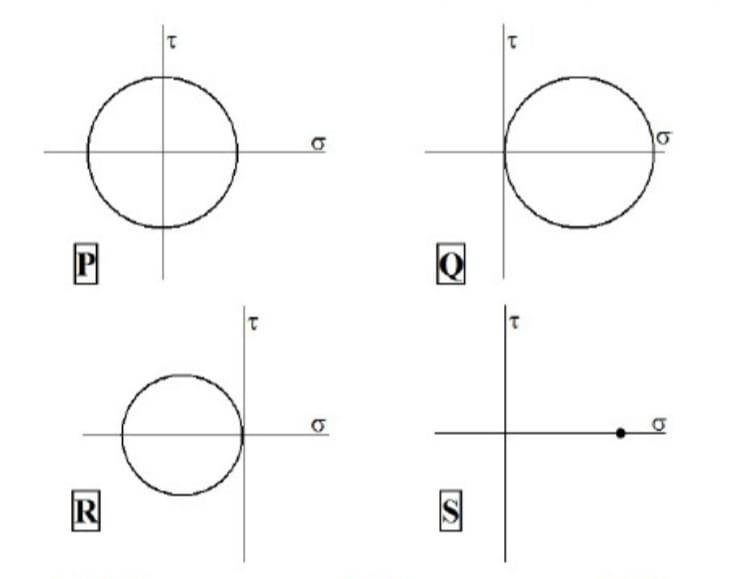
\includegraphics[width=0.6\textwidth]{images/q33i.jpg}
\end{center}
\begin{enumerate}[label=(\alph*)]
  \item P
  \item Q
  \item R
  \item S
\end{enumerate}

\item  Which statement is INCORRECT about the effect of small carbon addition to iron? (GATE 2015 MT)
\begin{enumerate}[label=(\alph*)]
  \item DBTT increases.
  \item Hardenability increases.
  \item Toughness increases.
  \item Yield point phenomenon occurs.
\end{enumerate}

\item  In polymers like epoxies, creep resistance is enhanced by (GATE 2015 MT)
\begin{enumerate}[label=(\alph*)]
  \item increasing bulkiness of side groups.
  \item increasing cross-link density.
  \item adding plasticizers.
  \item annealing.
\end{enumerate}











\item The value of eigenvalue for matrix A is given, find the other eigenvalues. (NAT question) (GATE 2015 MT)

\item Find the magnitude of gradient of function at point given. (NAT question) (GATE 2015 MT)

\item Determine the determinant of given matrix. (NAT question) (GATE 2015 MT)

\item The solution of given differential equation is: (GATE 2015 MT)
\begin{enumerate}[label=(\alph*)]
  \item $y = 5$
  \item $y = e^{5x}$
  \item $y = 2x$
  \item $y = 5x^2$
\end{enumerate}

\item Find the maximum value of function $f(x) = x^2 + 2x$. (NAT) (GATE 2015 MT)

\item Select the correct Gibbs free energy versus temperature plot from figure: (GATE 2015 MT)
\begin{center}
  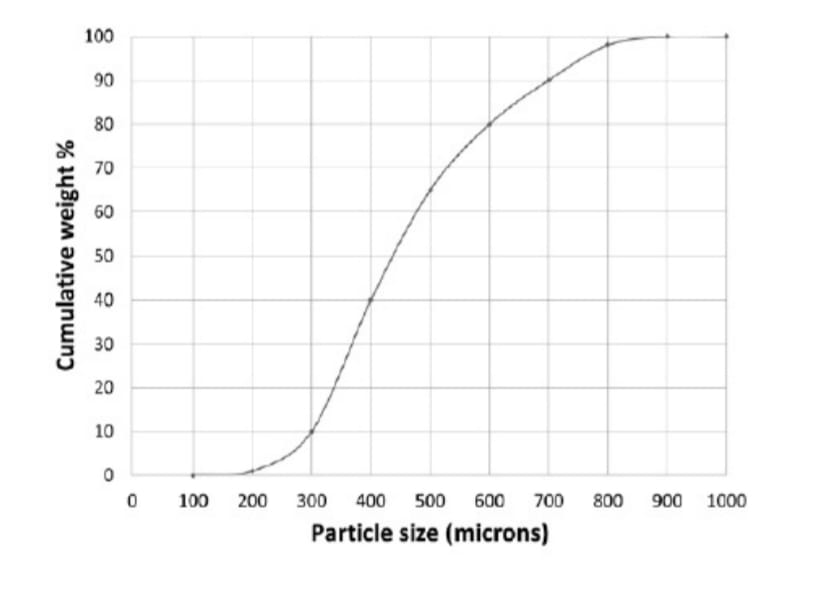
\includegraphics[width=0.6\textwidth]{images/q46i.jpg}
\end{center}
\begin{enumerate}[label=(\alph*)]
  \item A
  \item B
  \item C
  \item D
\end{enumerate}

\item Calculate equilibrium $P_{CO_2}/P_{CO}$ ratio for given reaction at temperature. (NAT question) (GATE 2015 MT)

\item Calculate the amount of ore required for producing pure metal. (NAT question) (GATE 2015 MT)

\item Determine pressure difference in manometer shown. (GATE 2015 MT)
\begin{center}
  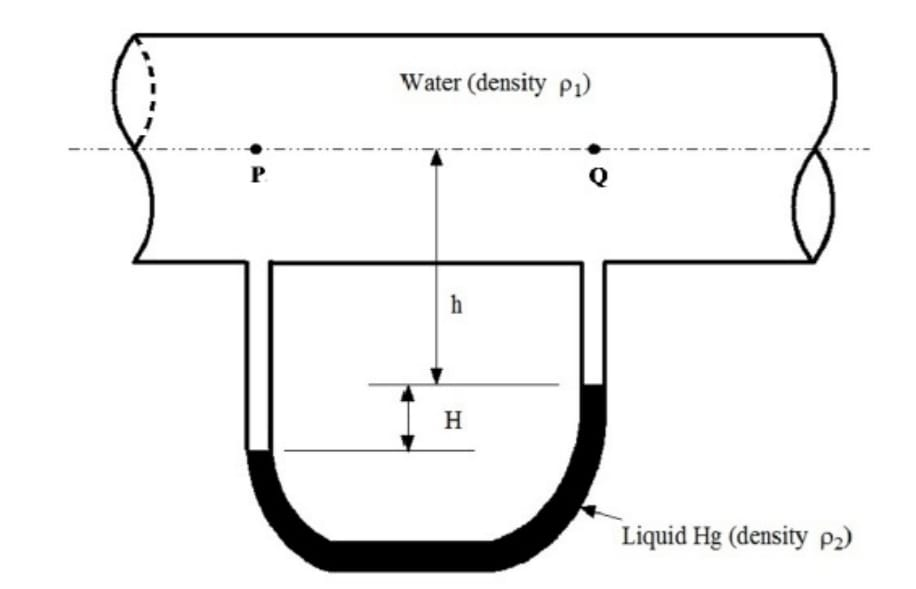
\includegraphics[width=0.6\textwidth]{images/q44i.jpg}
\end{center}
\begin{enumerate}[label=(\alph*)]
  \item $P_2 g H$
  \item $P_1 g h$
  \item $(\rho_2 - \rho_1) g H$
  \item $(P_2 - P_1) g h$
\end{enumerate}

\item Match metals in Group I with extraction routes in Group II: (GATE 2015 MT)
\begin{table}[h]
\centering
\begin{tabular}{|c|c|}
\hline
Group I & Group II \\
\hline
P. Al & 3. Electrolysis of fused salts\\
Q. Ti & 2. Matte smelting \\
R. Cu & 4. Halide metallurgy \\
S. Fe & 1. Blast furnace \\
\hline
\end{tabular}
\end{table}
\begin{enumerate}[label=(\alph*)]
  \item P-3, Q-2, R-4, S-1
  \item P-2, Q-4, R-3, S-1
  \item P-3, Q-4, R-2, S-1
  \item P-4, Q-1, R-3, S-2
\end{enumerate}

\item Particle size distribution after sieving (NAT question) (GATE 2015 MT)
\begin{center}
  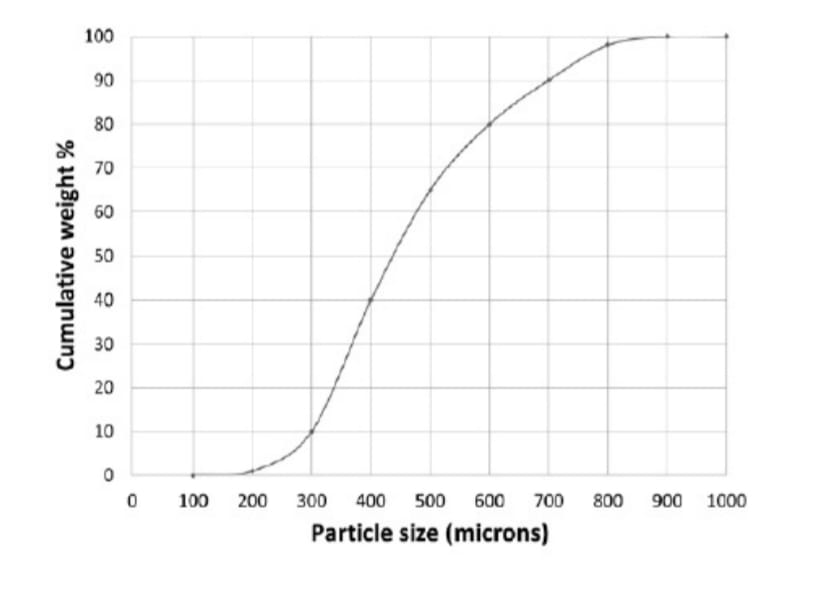
\includegraphics[width=0.6\textwidth]{images/q46i.jpg}
\end{center}

\item Calculate voltage in electrolytic refining. (NAT question) (GATE 2015 MT)

\item Configurational entropy maximum mole fraction (NAT question) (GATE 2015 MT)

\item Calculate free energy change on undercooling (NAT question) (GATE 2015 MT)

\item Match names in Group I with reactions in Group II: (GATE 2015 MT)
\begin{table}[h]
\centering
\begin{tabular}{|c|c|}
\hline
Group I & Group II \\
\hline
P. Eutectic & 2. $L \to \alpha + \beta$ \\
Q. Peritectic & 3. $L_1 \to L_2 + \alpha$ \\
R. Peritectoid & 1. $\gamma + \beta \to \alpha$ \\
S. Monotectic & 4. $L + \beta \to \alpha$ \\
\hline
\end{tabular}
\end{table}
\begin{enumerate}[label=(\alph*)]
  \item P-2, Q-3, R-1, S-4
  \item P-3, Q-4, R-1, S-2
  \item P-2, Q-4, R-1, S-3
  \item P-4, Q-1, R-3, S-2
\end{enumerate}

\item Time to homogenize alloy at different temperature (NAT question) (GATE 2015 MT)

\item Match materials in Group I with applications in Group II: (GATE 2015 MT)
\begin{table}[h]
\centering
\begin{tabular}{|c|c|}
\hline
Group I & Group II \\
\hline
P. Iron-Silicon alloy & 3. Transformer core \\
Q. GaAs & 4. Light emitting diode \\
R. Nichrome & 1. Heating element \\
S. Quartz crystals & 2. Ultrasonic generator \\
\hline
\end{tabular}
\end{table}
\begin{enumerate}[label=(\alph*)]
  \item P-3, Q-4, R-1, S-2
  \item P-1, Q-3, R-4, S-2
  \item P-2, Q-4, R-1, S-3
  \item P-3, Q-2, R-4, S-1
\end{enumerate}

\item Match heat treatment microstructures for eutectoid steel (GATE 2015 MT)
\begin{center}
  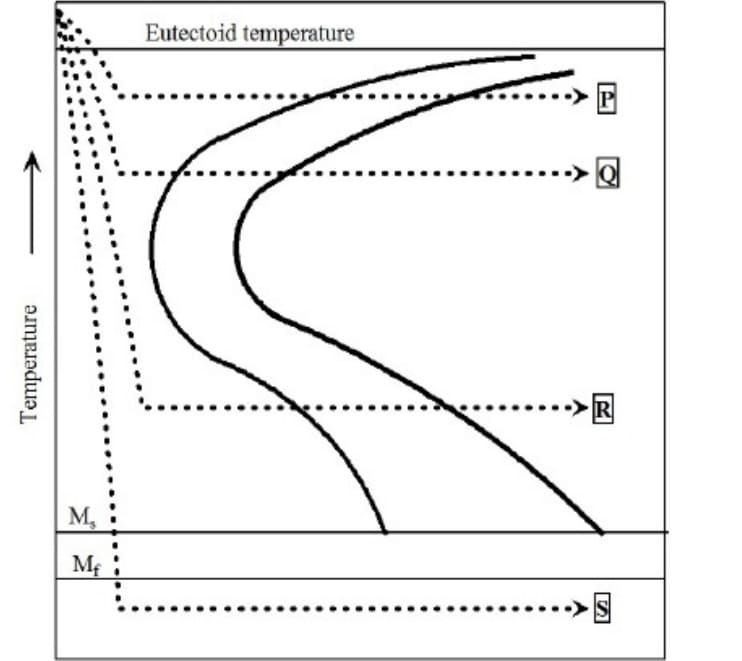
\includegraphics[width=0.7\textwidth]{images/q53i.jpg}
\end{center}
\begin{tabular}{|c|c|}
\hline
P & Fine pearlite \\
Q & Martensite \\
R & Bainite \\
S & Coarse pearlite \\
\hline
\end{tabular}
\begin{enumerate}[label=(\alph*)]
  \item P-1, Q-2, R-4, S-3
  \item P-4, Q-1, R-3, S-2
  \item P-2, Q-4, R-1, S-3
  \item P-1, Q-4, R-3, S-2
\end{enumerate}

\item Microstructure phase diagram question (NAT) (GATE 2015 MT)
\begin{center}
  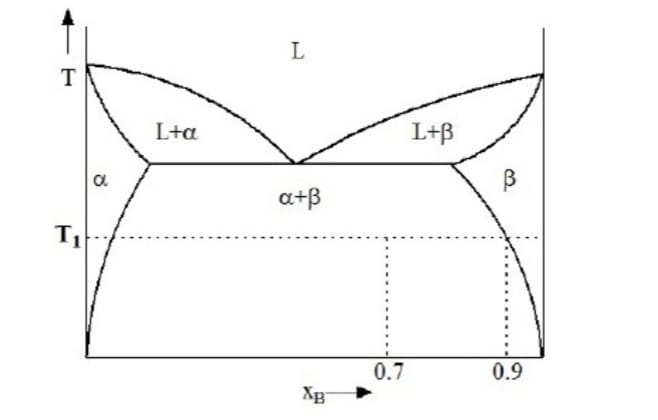
\includegraphics[width=0.6\textwidth]{images/q54i.jpg}
\end{center}

\item Calculate diameter of forged pancake (NAT question) (GATE 2015 MT)

\item Correctness of assertion and reason (GATE 2015 MT)
\begin{enumerate}[label=(\alph*)]
  \item Both are true, reason is correct
  \item Both are true, reason incorrect
  \item Both are false
  \item Assertion true, reason false
\end{enumerate}

% Continue up to question 65 continuing similar formatting...

\item Metal mass flow rate issue (NAT) (GATE 2015 MT)

\item Match defects with their cause in castings (GATE 2015 MT)
\begin{table}[h]
\centering
\begin{tabular}{|c|c|}
\hline
Group I & Group II \\
\hline
P. Macrosegregation & 4. Density difference and convection \\
Q. Fine grained structure & 1. Inoculation \\
R. Porosity & 2. Gas evolution and shrinkage \\
S. Dendrites & 3. Temperature gradients and supercooling \\
\hline
\end{tabular}
\end{table}
\begin{enumerate}[label=(\alph*)]
  \item P-1, Q-3, R-2, S-4
  \item P-4, Q-1, R-2, S-3
  \item P-2, Q-4, R-1, S-3
  \item P-4, Q-1, R-3, S-2
\end{enumerate}

\item Driving force for sintering particle size reduction (NAT) (GATE 2015 MT)

\item Detecting internal flaws in ceramic materials - NOT applicable techniques (GATE 2015 MT)
\begin{enumerate}[label=(\alph*)]
  \item Liquid penetration and ultrasonic testing
  \item Ultrasonic testing and eddy current
  \item Radiography and eddy current
  \item Liquid penetration and eddy current
\end{enumerate}

\item Match fracture surface features with mechanisms (GATE 2015 MT)
\begin{table}[h]
\centering
\begin{tabular}{|c|c|}
\hline
Group I & Group II \\
\hline
P. Striations & 4. Fatigue fracture \\
Q. Dimples and microvoids & 3. Ductile fracture \\
R. Flat facets and river markings & 2. Cleavage fracture \\
S. Jagged surface with grain-like features & 1. Intergranular fracture \\
\hline
\end{tabular}
\end{table}
\begin{enumerate}[label=(\alph*)]
  \item P-1, Q-2, R-3, S-4
  \item P-1, Q-3, R-2, S-4
  \item P-4, Q-3, R-2, S-1
  \item P-2, Q-1, R-4, S-3
\end{enumerate}

\item Match scientist pairs with phenomena (GATE 2015 MT)
\begin{table}[h]
\centering
\begin{tabular}{|c|c|}
\hline
Group I & Group II \\
\hline
P. Hall-Petch & 4. Grain boundary strengthening \\
Q. Nabarro-Herring & 2. Diffusional creep \\
R. Lomer-Cottrell & 1. Dislocation reaction product \\
S. Frank-Read & 3. Dislocation source \\
\hline
\end{tabular}
\end{table}
\begin{enumerate}[label=(\alph*)]
  \item P-1, Q-2, R-3, S-4
  \item P-1, Q-2, R-4, S-3
  \item P-4, Q-2, R-1, S-3
  \item P-4, Q-1, R-2, S-3
\end{enumerate}

\item In an FCC crystal, the strain energy per unit length of a dislocation with Burgers vector $b = \frac{a}{2} (110)$ is ______ times that of $\frac{a}{6} (112)$ dislocation. (NAT) (GATE 2015 MT)

\item Match mechanical properties with microstructural features (GATE 2015 MT)
\begin{table}[h]
\centering
\begin{tabular}{|c|c|}
\hline
Group I & Group II \\
\hline
P. Creep resistance & 3. Coherent precipitates \\
Q. Elastic modulus enhancement & 4. Glass fibres in epoxy \\
R. Superplasticity & 2. Single crystal \\
S. Increased strength & 1. Fine grained two-phase microstructure \\
\hline
\end{tabular}
\end{table}
\begin{enumerate}[label=(\alph*)]
  \item P-3, Q-4, R-2, S-1
  \item P-1, Q-2, R-3, S-4
  \item P-2, Q-4, R-1, S-3
  \item P-1, Q-4, R-2, S-3
\end{enumerate}

\item A brittle material has surface energy $\gamma_1 = 0.9$ J/m$^2$ and fracture strength 300 MPa in medium P. Tested in medium Q with $\gamma_2 = 0.1$ J/m$^2$, the fracture strength (MPa) in medium Q based on Griffith’s theory is ________. (NAT) (GATE 2015 MT)

\end{enumerate}


\end{document}